\documentclass{article}
\usepackage[margin=1in, top = .8in, left=.8in]{geometry}
\usepackage{comment}
\usepackage{amsmath, amssymb}
\usepackage{framed}
\usepackage{enumerate}
\usepackage{comment}
\usepackage{tikz,pgfplots}
\usepgfplotslibrary{fillbetween}
\pgfplotsset{compat=1.15}
\usepackage[hyphens]{url}

\newcommand{\fgraff}{
\begin{minipage}[l][.30\textwidth]{3 in}{
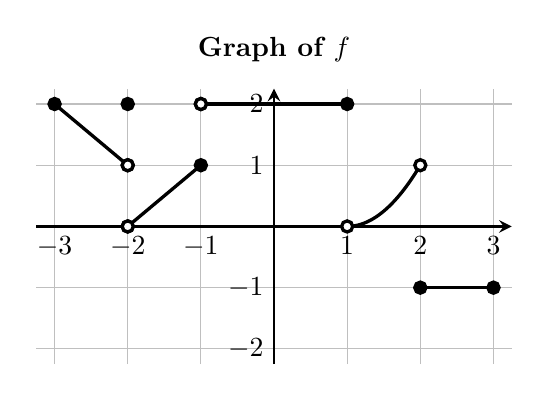
\begin{tikzpicture}
\begin{axis}[
   	xmin=-3.25, xmax=3.25,
	ymin=-2.25, ymax=2.25,
	major tick length={0},
	xtick={-3,-2,...,3}, ytick={-2,-1,...,2},
	line width=1pt, title={\textbf{Graph of $f$}},
 	axis lines=center, height=2 in, width=3 in, grid=major,
 	restrict y to domain=-2.25:2.25
	]
	\addplot [mark=*, black, smooth, very thick] plot coordinates {(-3,2)(-2,1)};
	\addplot [mark=*, black, smooth, very thick] plot coordinates {(-2,3)};
	\addplot [mark=*, black, smooth, very thick] plot coordinates {(-2,0)(-1,1)};
	\addplot [mark=*, black, smooth, very thick] plot coordinates {(-1,2)(1,2)};
	\addplot [mark=*, black, smooth, very thick] plot coordinates {(2,-1)(3,-1)};
    \addplot [black, smooth, very thick, samples=100, domain=1:2] {(x-1)^2};
    \addplot [black, only marks, very thick, mark=*, mark options={scale=1, fill=white}]
    coordinates{(1,0) (2,1) (-1,2) (-2,1) (-2,0)};
    \addplot [black, only marks, very thick, mark=*] coordinates{(-2,2)};
\end{axis}
\end{tikzpicture}
%\end{center}
}
\end{minipage}}

\newcommand{\ggraff}{
\begin{minipage}[l][.30\textwidth]{3 in}{
%\begin{center}
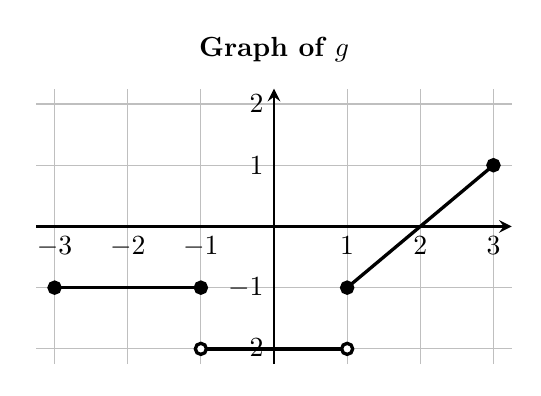
\begin{tikzpicture}
\begin{axis}[
   	xmin=-3.25, xmax=3.25,
	ymin=-2.25, ymax=2.25,
	major tick length={0},
	xtick={-3,-2,...,3}, ytick={-2,-1,...,2},
	line width=1pt, title={\textbf{Graph of $g$}},
 	axis lines=center, height=2 in, width=3 in, grid=major,
 	restrict y to domain=-2.25:2.25
	]
	\addplot [mark=*, black, smooth, very thick] plot coordinates {(-3,-1)(-1,-1)};
	\addplot [mark=*, black, smooth, very thick] plot coordinates {(1,-1)(3,1)};
	\addplot [black, very thick, mark=*, mark options={scale=1, fill=white}] plot coordinates {(-1,-2)(1,-2)};
\end{axis}
\end{tikzpicture}
%\end{center}
}
\end{minipage}}

\begin{document}
\begin{center}
    \large \textbf{Homework 1}
\end{center}
%\begin{itemize}
%    \item[\textbf{Week 1}]
        \begin{itemize}
            %\item Prerequisite Content:
            \item Part 1
                \begin{enumerate}
                    \item For each of the following, solve for the stated variable or expression.
                        \begin{enumerate}
                            \item $\displaystyle \frac{x}{1-x}=b$; solve for $x$ in terms of $b$.
                            \item $\displaystyle \left( \frac{x}{1-x}\right)\bigg/\left(\frac{p}{1-p}\right) = b$; solve for $x$ in terms of $p$ and $b$.
                            \item $\displaystyle \left(\frac{x}{1-x}\right) \bigg/ \left(\frac{p}{1-p}\right) = \exp(b) = e^b$; solve for $x$ in terms of $p$ and $b$.
                            \item $\displaystyle \exp(a)\exp(b)\exp(c)=\exp(x)$; solve for $x$ in terms of $a$, $b$, and $c$.
                            \item Suppose $\displaystyle p_0 = \frac{\exp(a+bx)}{1+\exp(a+bx)}$ and suppose $\displaystyle p_1=\frac{\exp(a+b(x+1))}{1+\exp(a+b(x+1))}$.  Write $\displaystyle \left(\frac{p_1}{1-p_1}\right) \bigg/ \left(\frac{p_0}{1-p_0}\right)$ in terms of $a$, $b$, and $x$.
                            \item $\displaystyle y_1-(mx_1+b)+y_2-(mx_2+b)+y_3-(mx_3+b)+y_4-(mx_4+b)+y_5-(mx_5+b)=0$; solve for $b$ in terms of the $x_i's$, $y_i's$, and $m$.
                        \end{enumerate}
                    \item Find the value of $c$ that makes the following identity hold. $$\frac{(k-np)^2}{np}+\frac{((n-k)-n(1-p))^2}{n(1-p)}=\frac{(k-np)^2}{c}$$
                    \item Solve the following inequality for $n$ $$1-\left(\frac{\sigma}{t}\right)^2 \geq 0.99$$ when $t=0.05$ and $\displaystyle \sigma = \frac{1.5}{\sqrt{n}}$.
                    \item Let $\sigma >0$ and $q >0$.  Consider the statement $\displaystyle \frac{x-\mu}{\sigma} \in (-q, q)$, which is equivalent the the following inequality: $$-q < \frac{x-\mu}{\sigma} <q.$$  Find a value $a$ that depends on $\mu$, $\sigma$, and $q$, such that the inequality above implies that $x\in(-a,a)$. 
                \end{enumerate}
            %\item Async (Week 1):
            \item Part 2
                \begin{enumerate}
                    \item Complete the square of the expression $$-\frac{1}{2}(a\mu^2-2b\mu)$$  In other words, write the expression in the form $c(\mu-d)^2+k$.
                    \item In statistics, the mean ($\mu$) of a set of numbers $\{x_1, x_2, \cdots, x_n\}$ is given by the formula $$\mu = \frac{1}{n}\sum_{k=1}^n x_k$$  Show that $$\frac{1}{n}\sum_{k=1}^n (x_k-\mu)^2 = \frac{1}{n}\sum_{k=1}^n x_k^2-\mu^2$$  FYI: The equation above demonstrates two expressions for variance, where the one on the right side is often considered an improvement for computational purposes.  You will use this improvement on the formula for variance in both the second foundations and the probability courses.
                    \item The following two equations will be encountered later in this course as part of a larger problem of finding maximum values of a multivariable function.  Solve each equation for the variable indicated. 
                       \begin{enumerate}
                           \item $\displaystyle \frac{1}{\sigma^2}\sum_{k=1}^{n}(x_k-\mu)=0$; solve for $\mu$.
                           \item $\displaystyle -\frac{n}{\sigma}+\frac{1}{\sigma^3}\sum_{k=1}^{n}(x_k-\mu)^2=0$; solve for $\sigma$.
                       \end{enumerate} 
                    \item  Solve for $p$. (Note that in order to simplify the notation, $\displaystyle \sum_{i=0}^n x_i$ has been abbreviated as  $\sum x_i$.) $$\displaystyle \frac{\sum x_i }{p} - \frac{n-\sum x_i}{p-1}=0 $$
                    \item Consider the function $\displaystyle p(x) = \frac{1}{\sqrt{2\pi \sigma^2}}\exp\left( \frac{-(x-\mu)^2}{2\sigma^2}\right)$, which is the normal probability density function.  Let $h(x) = \ln(p(x))$.  Express $h(x)$ as a quadratic so it is of the form $ax^2+bx+c$. What are $a,b,$ and $c$? 
                    \item Suppose that $\displaystyle f(i)= e^{-\lambda}\frac{\lambda^i}{(i+1)!}$.  Calculate $\displaystyle \frac{f(i+1)}{f(i)}$, and fully simplify.
                    \item Consider the functions $\displaystyle g_1(x) = \frac{x^2-1}{x-1}$ and $\displaystyle g_2(x)= x+1$. Explain why $g_1(x) \neq g_2(x)$.
                    \item Say that $p(i)$ is defined below:
                        $$ p(i) = \begin{cases} 
                        c\cdot i & \text{if $1 
                        \leq i \leq 20, \quad i \in N$} \\
                        0 & \text{otherwise} \\
                        \end{cases}
                        $$
                        Find the value of the constant $c$ so that $\displaystyle \sum_{i=1}^{20} p(i)$ = 1. Then, using that value of $c$, find $\displaystyle \sum_{i=1}^{20} i\cdot p(i)$ and $\displaystyle \sum_{i=1}^{20} i^2 \cdot p(i)$. 
                    \item In probability you will use the notation $\displaystyle n\choose k$ (pronounced ``n choose k''). These numbers are called the binomial coefficients and can be found by the formula ${n\choose k} = \frac{n!}{k!(n-k)!}$. For example, ${5 \choose 3}= \frac{5!}{3!\cdot2!}=\frac{5\cdot 4\cdot 3 \cdot 2 \cdot 1}{(3\cdot 2 \cdot 1) (2 \cdot 1)} = \frac{5\cdot4}{2\cdot 1} = 10$.
                        \begin{enumerate}
                            \item Calculate $\displaystyle {6 \choose 4}$.
                            \item Calculate $\displaystyle \sum_{k=0}^6 {6\choose k}$.
                            \item Guess a formula for $\displaystyle \sum_{k=0}^n {n\choose k}$.
                        \end{enumerate}
                    \item Construct a function $m:\mathbb{R}^2 \rightarrow \mathbb{R}$ that inputs two numbers $x$ and $y$ that outputs the minimum of $x$ and $y$.  (You are allowed to use the following operations to construct your function: addition, subtraction, multiplication, division, absolute value, square roots, exponentiation, and log.) \\  Show that your choice of function works by first assuming that $x\geq y$ and showing that the function outputs $y$ and then assuming that $x \leq y$ and showing that the function outputs $x$.
                    \item Write each of the following expressions using summation notation.
                        \begin{enumerate}
                            \item $\displaystyle \frac{1}{3}+\frac{1}{9}+\frac{1}{27}+\frac{1}{81} + \frac{1}{243}+ \frac{1}{729}$
                            \item $\displaystyle \frac{5^2}{2!}+\frac{5^3}{3!}+\frac{5^4}{4!} + \cdots + \frac{5^{19}}{19!}$
                            \item $2^{i_1} + 2^{i_2} + \ldots 2^{i_k}$
                        \end{enumerate}
                \end{enumerate}
        \end{itemize}










  

 

%\end{itemize}
\end{document}
